\chapter{Phase 2 - Industrial Safety Detection}
\setcounter{section}{0}
\renewcommand{\thesection}{\arabic{section}}
\label{chap:industrial-safety}

\section*{Introduction}
This chapter presents the technical background and implementation work for the industrial safety capabilities within the EYE-D video analytics solution. The focus of this chapter is strictly on object \textbf{Detection} in complex industrial environments. The primary industrial hazards addressed are fire, smoke, and forklift collisions, which pose immediate existential threats to both personnel and infrastructure.

Detecting these hazards reliably requires a highly optimized inference model capable of running natively on edge Neural Processing Units (NPUs). These target hardware platforms impose strict constraints on memory footprint, thermal output, and computational complexity (GFLOPs). Consequently, large-scale transformer models are often impractical for real-time edge deployment. This constraint dictates the need for highly efficient, single-stage detection architectures.

\section{Targeted State of the Art: The YOLO Family (v5 \& v8)}
To satisfy the strict efficiency-to-accuracy ratio demanded by NPU deployment, this project leverages the YOLO (You Only Look Once) family of models. Large-scale transformer architectures, while highly accurate, exceed the memory and compute limits of edge devices. The YOLO family provides a spectrum of models, but it was explicitly determined that only the "Nano" models (YOLOv5n and YOLOv8n) were chosen to fit within the severely constrained NPU memory buffers (SRAM) without causing thermal throttling or out-of-memory errors.

\subsection{Architectural Evolution for Efficiency}
The evolution from YOLOv5 to YOLOv8 introduced several architectural shifts directly impacting edge deployment.

\subsubsection{Memory Efficiency: C3 vs. C2f Modules}
The backbone of these models relies on cross-stage partial bottlenecks. The key difference lies in how feature information flows through the module:

\begin{itemize}
  \item \textbf{C3 (YOLOv5)}: splits the input into two branches, passes one through a sequence of Bottleneck blocks, and concatenates the outputs. Uses 3 convolutional layers.
  \item \textbf{C2f (YOLOv8)}: splits the input and passes it through Bottleneck blocks, but \emph{concatenates the outputs of all intermediate Bottleneck stages} with the split input. Uses 2 convolutional layers.
\end{itemize}

This C2f-versus-C3 difference is detailed in Figure~\ref{fig:c2f-vs-c3}, which highlights the richer intermediate feature concatenation used by C2f.

\begin{figure}[H]
\centering
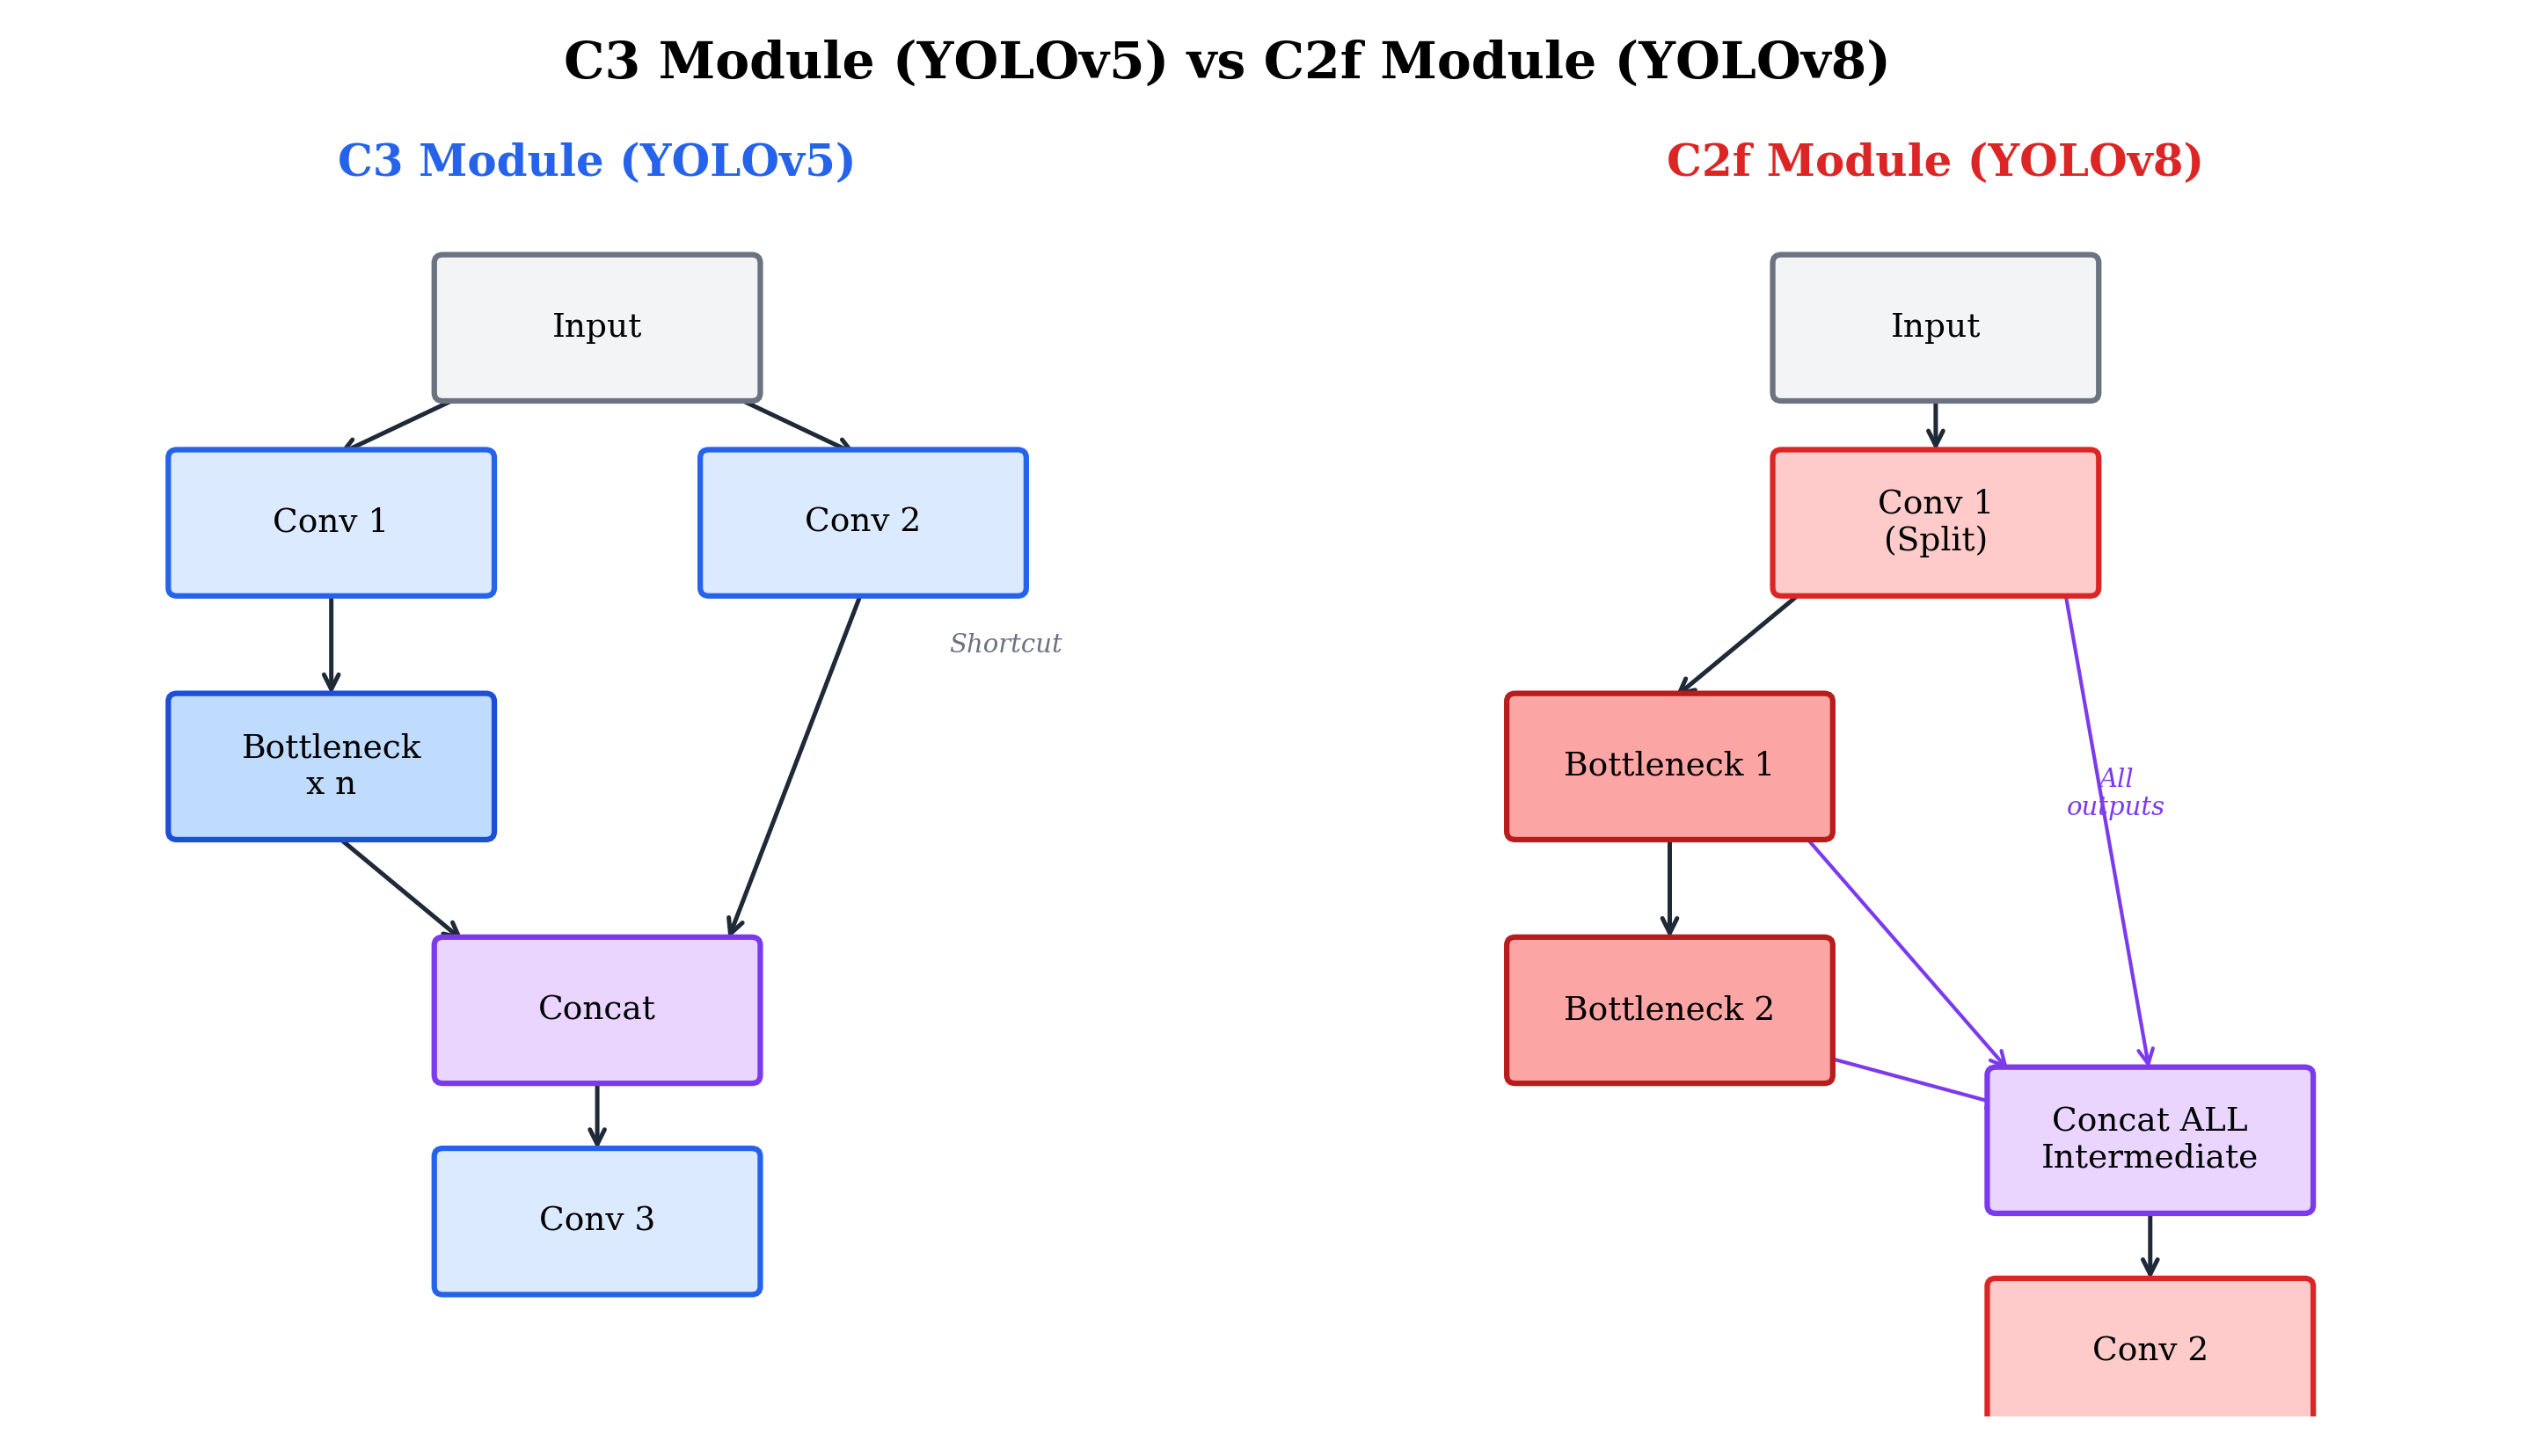
\includegraphics[width=0.95\textwidth]{diagrams/fig6_c2f_vs_c3.png}
\caption{C2f versus C3 module comparison}
\label{fig:c2f-vs-c3}
\end{figure}

While C2f provides richer gradient flow, it concatenates intermediate outputs from all Bottleneck stages, increasing peak memory consumption during inference. This makes YOLOv5's C3 module more memory-efficient for ultra-edge NPU deployments.

\subsubsection{Detection Head: Coupled vs. Decoupled Design}
Unlike YOLOv5's coupled head, YOLOv8 employs a decoupled design (Figure~\ref{fig:decoupled-head}) with separate branches for classification and regression.

\begin{figure}[H]
\centering
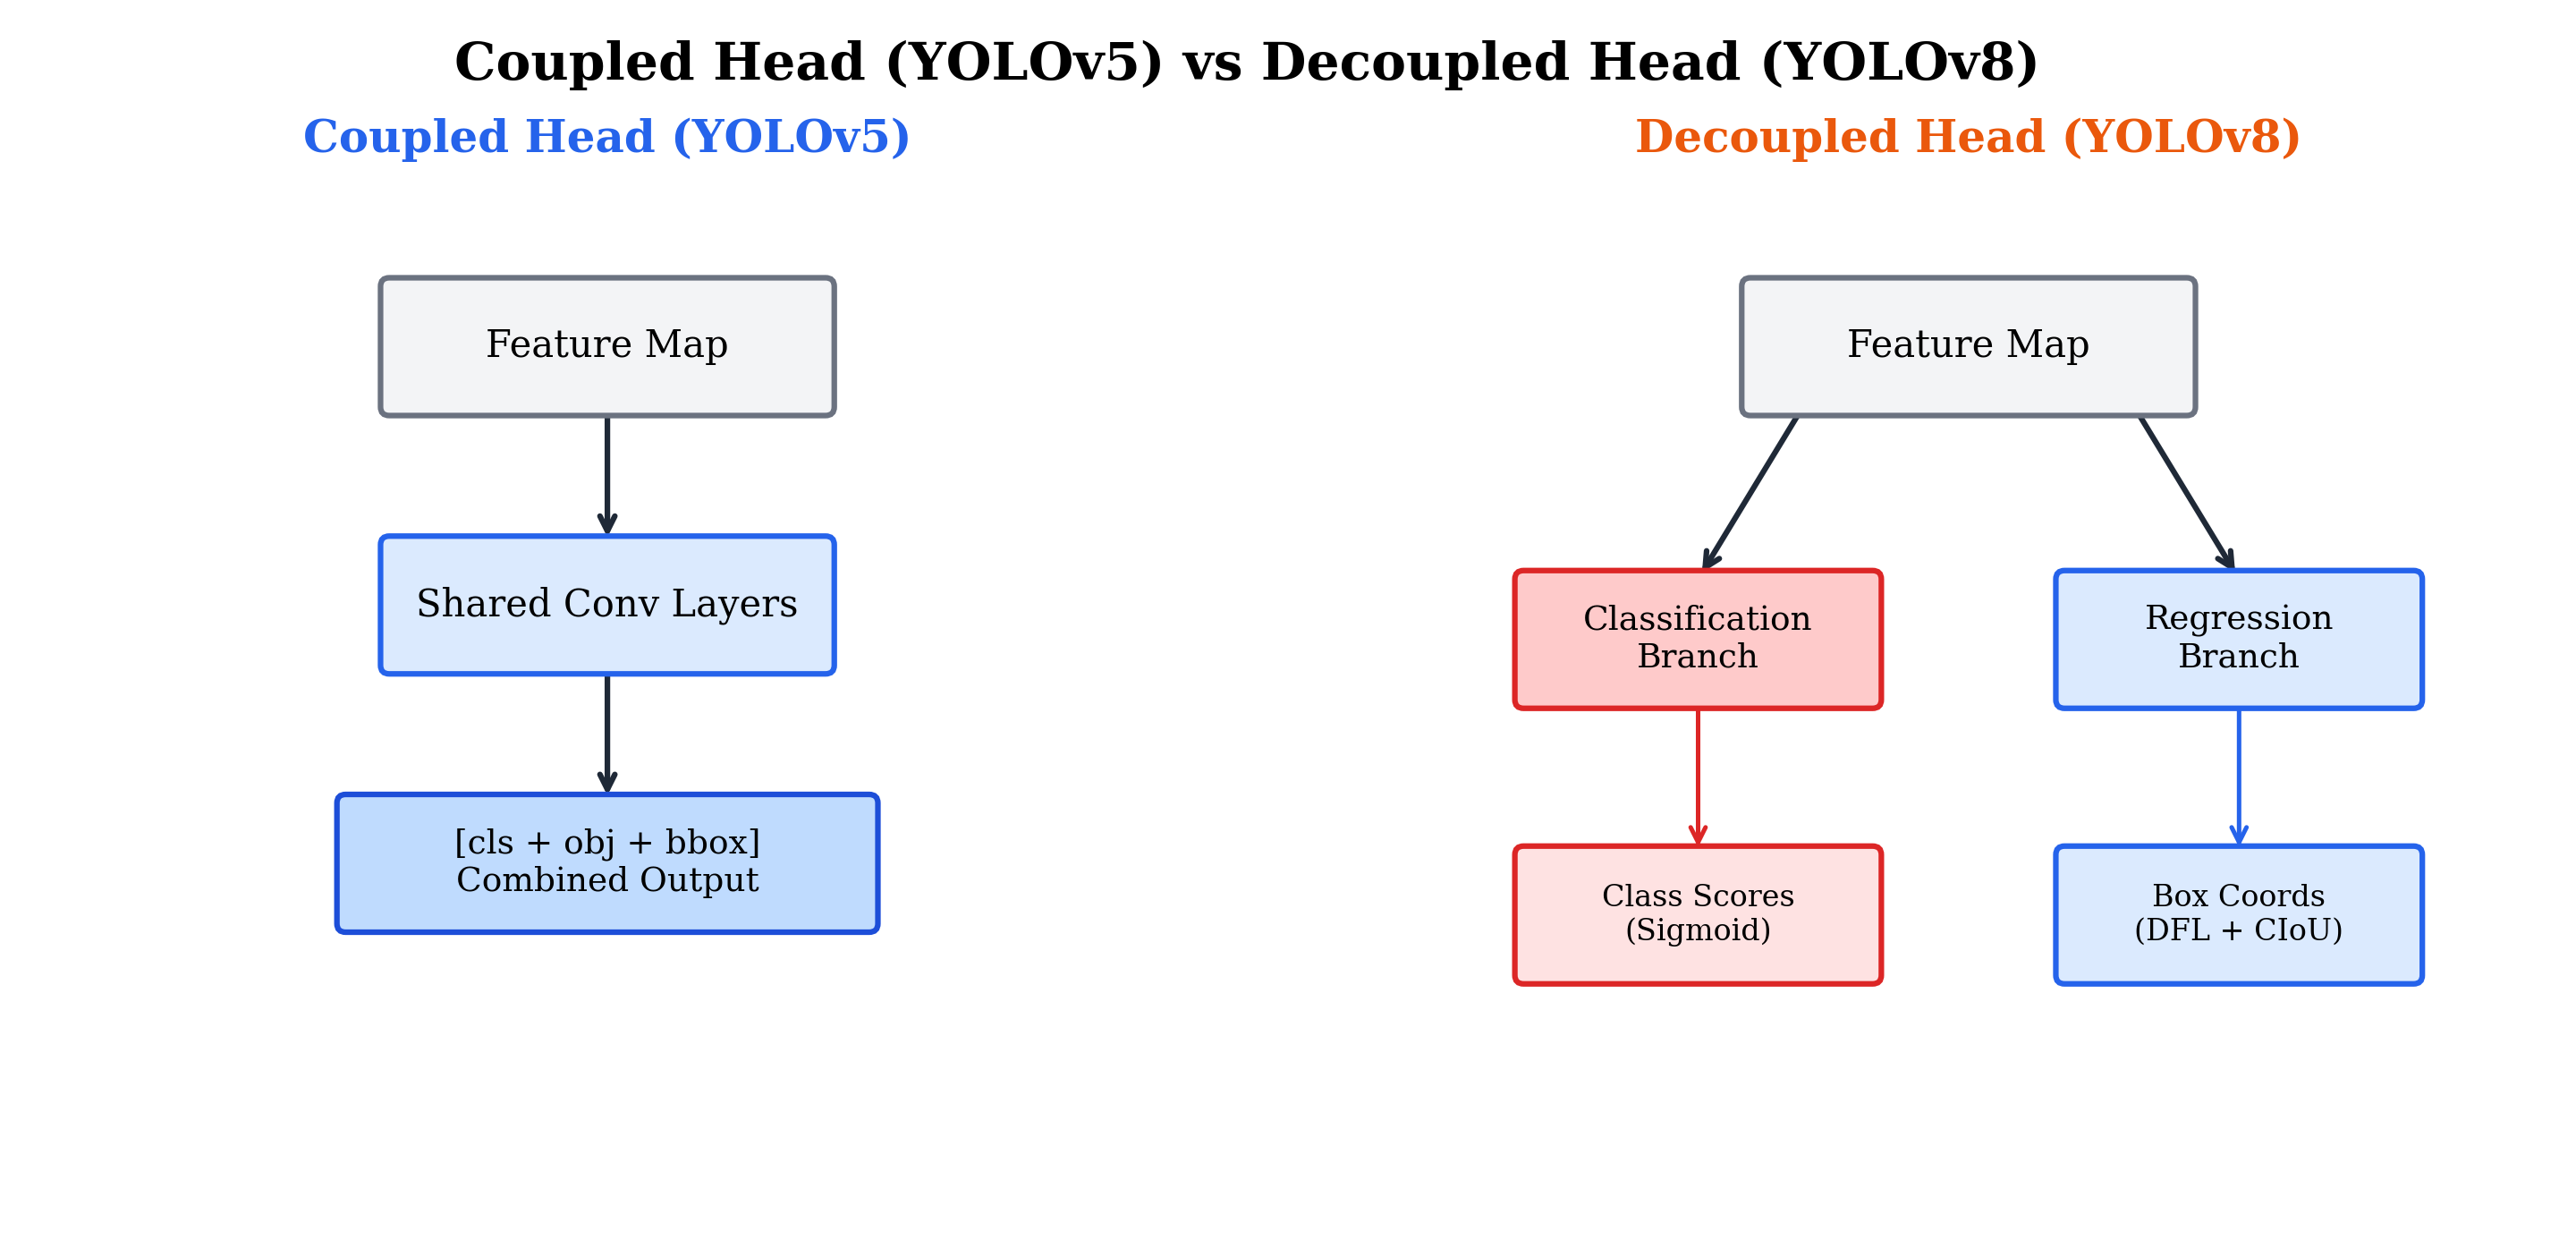
\includegraphics[width=0.85\textwidth]{diagrams/fig7_decoupled_head.png}
\caption{Decoupled versus coupled detection heads}
\label{fig:decoupled-head}
\end{figure}

The decoupled design addresses the conflict between classification and localization objectives. Separating the branches allows each to specialize, which is crucial for multi-class detection (like Fire and Smoke). However, for single-class detection (like Forklifts), YOLOv5's coupled head provides the necessary functionality with fewer parameters and FLOPs.

\subsection{Synthesis: Computational Efficiency and Resource Constraints}
The most direct comparison concerns the computational footprint of the nano variants, which are the primary deployment targets for NPU-based systems.

\begin{center}
\renewcommand{\arraystretch}{1.3}
\begin{tabular}{|p{0.20\textwidth}|p{0.14\textwidth}|p{0.14\textwidth}|p{0.14\textwidth}|p{0.22\textwidth}|}
\hline
\textbf{Metric} & \textbf{YOLOv5n} & \textbf{YOLOv8n} & \textbf{Difference} & \textbf{Advantage} \\
\hline
Parameters & 1.76M & 3.2M & $-$45\% & YOLOv5n \\
\hline
FLOPs & 4.1B & 8.7B & $-$53\% & YOLOv5n \\
\hline
Model Size & 3.56MB & 6.3MB & $-$43\% & YOLOv5n \\
\hline
CPU Inference & 73.6ms & 80.4ms & $-$8.5\% & YOLOv5n \\
\hline
GPU Inference (T4) & 0.6ms & 0.99ms & $-$39\% & YOLOv5n \\
\hline
\end{tabular}
\captionof{table}{YOLOv5n versus YOLOv8n compute comparison}
\label{tab:v5n-vs-v8n-compute}
\end{center}

YOLOv5n requires 45\% fewer parameters and 53\% fewer FLOPs than YOLOv8n. The computational cost difference between YOLOv5 and YOLOv8 is illustrated by comparing FLOPs across matching variants in Figure~\ref{fig:flops-comparison}.

\begin{figure}[H]
\centering
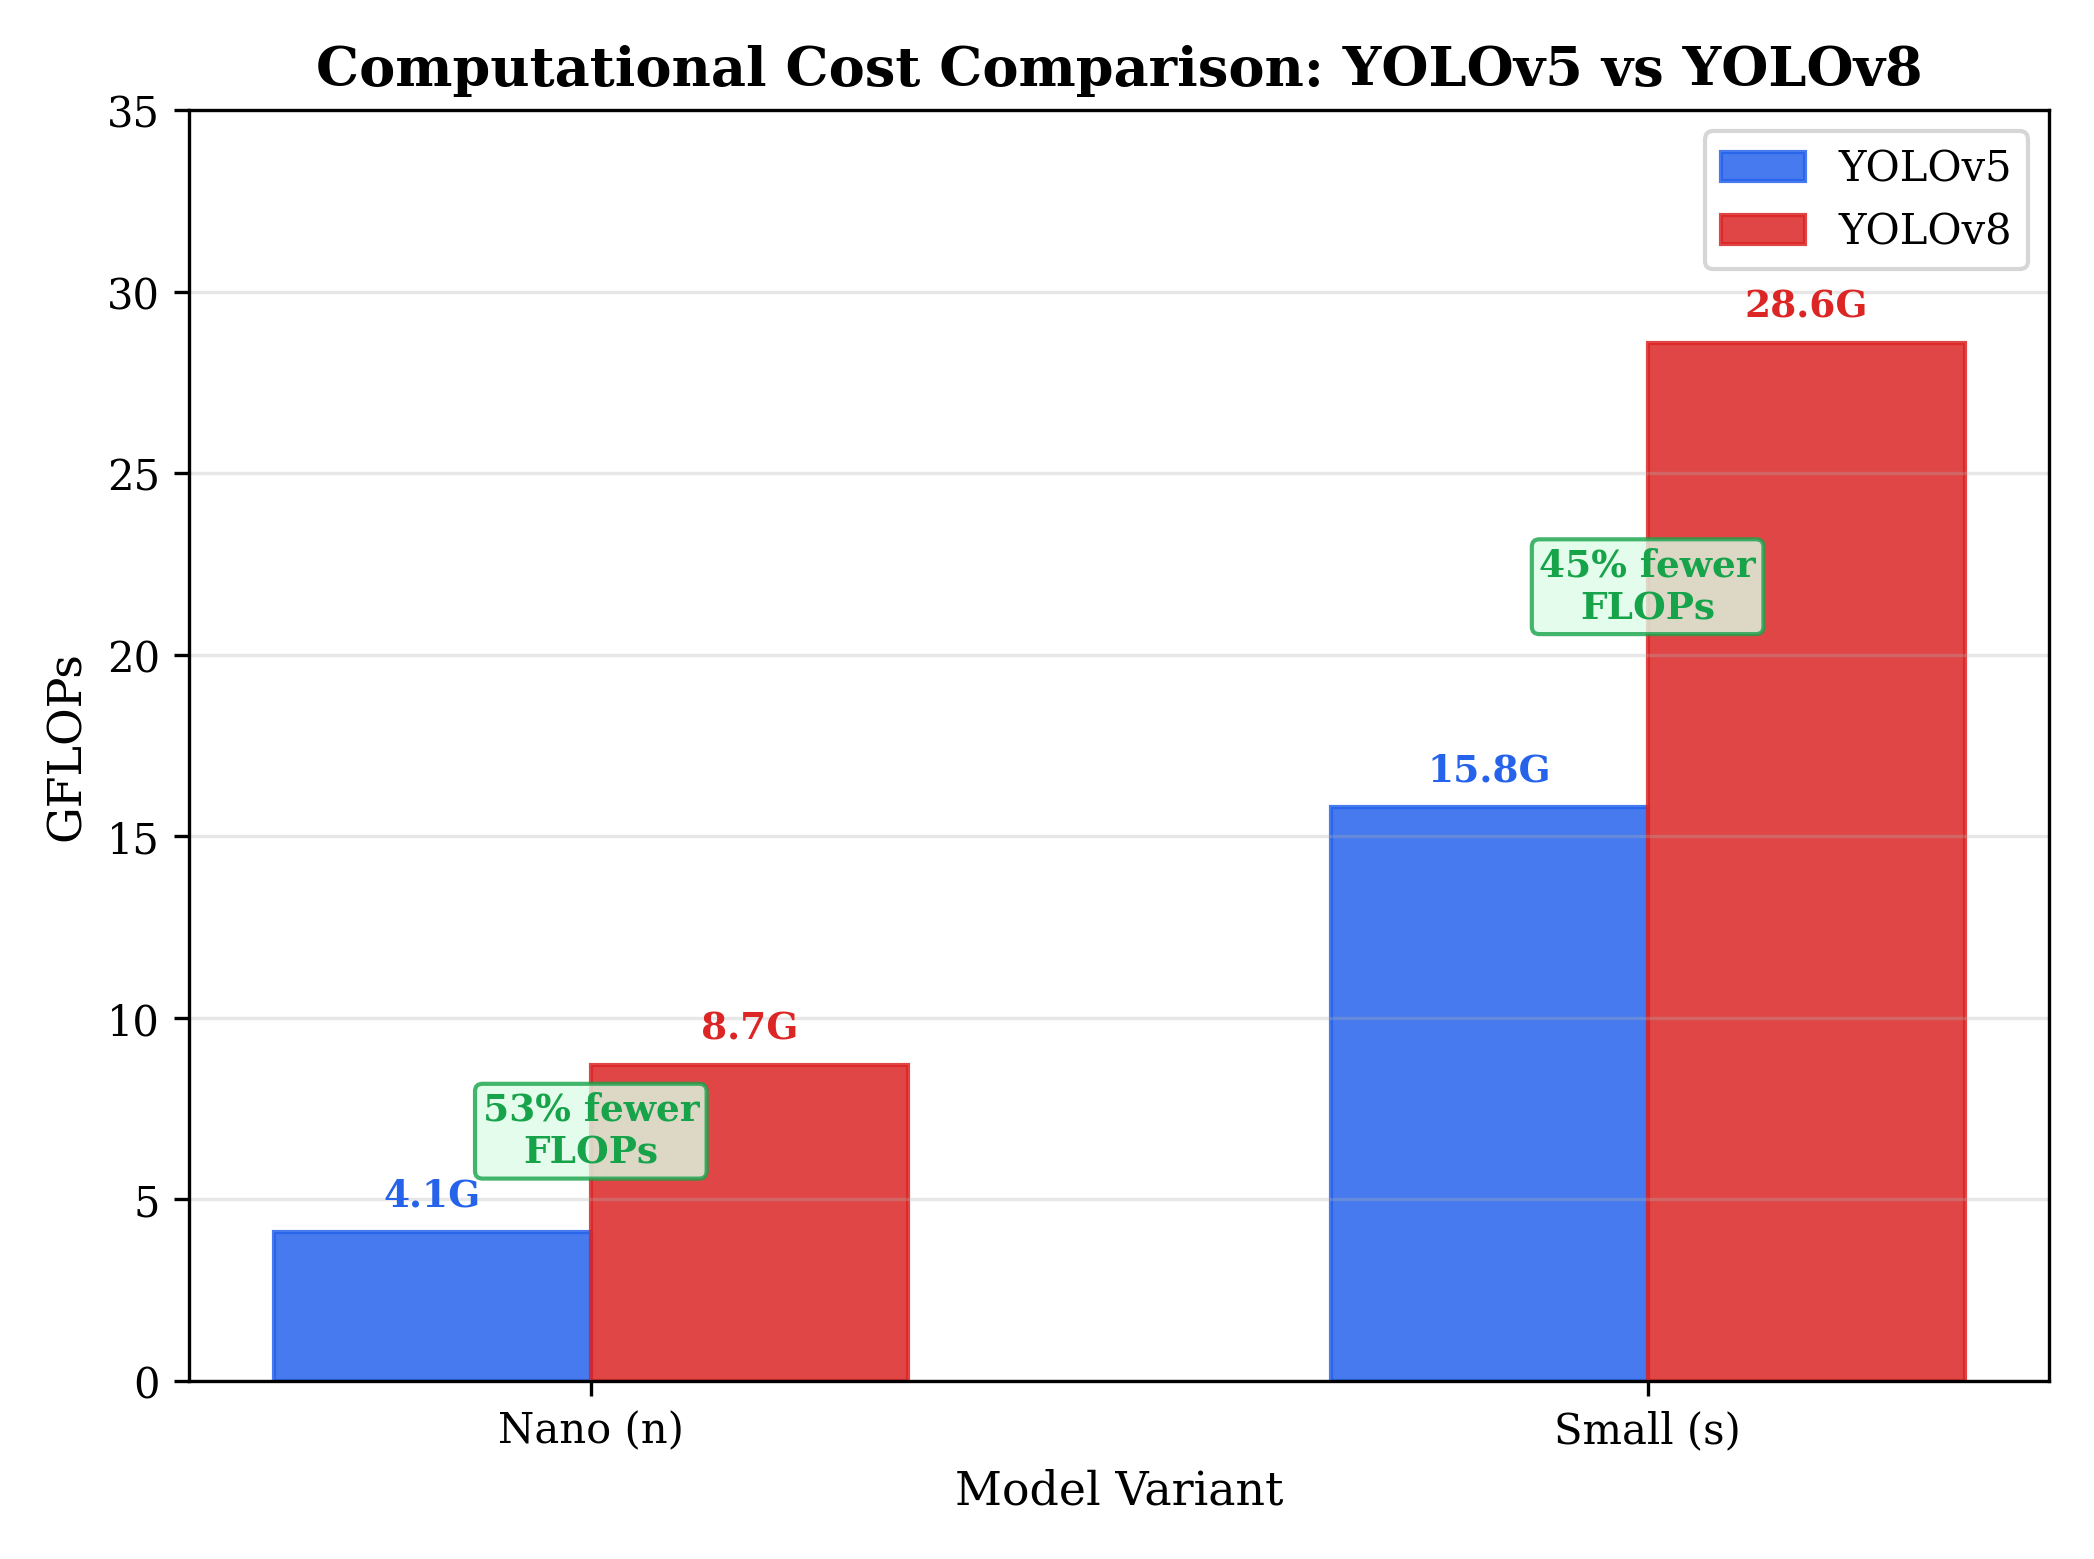
\includegraphics[width=0.85\textwidth]{diagrams/fig11_flops_comparison.png}
\caption{FLOPs comparison of YOLOv5 and YOLOv8}
\label{fig:flops-comparison}
\end{figure}

\textbf{Conclusion for EYE-D:} The selection between YOLOv5n and YOLOv8n was driven by aligning the model's architectural strengths with the task's complexity. YOLOv5n (Anchor-based, Coupled Head, lowest FLOPs) was selected for Forklifts, as it is optimal for rigid, single-class objects with predictable aspect ratios, maximizing efficiency. YOLOv8n (Anchor-free, Decoupled Head, C2f modules) was selected for Fire/Smoke, as it provides higher accuracy for dynamic, semi-transparent objects with unpredictable shapes, fully utilizing the NPU compute budget.

\section{Implementation: Fire and Smoke Detection}
\label{sec:fire-smoke-implementation}

The core component of this phase focuses on early hazard detection, specifically identifying fire and smoke. This implementation prioritizes real-time alerting while drastically reducing false positives (e.g., misclassifying steam, reflections, or intense industrial lighting as fire).

\subsection{Training Parameters and Dataset Composition}
The YOLOv8n (nano) architecture was selected for this task due to its advanced multi-scale feature extraction capability (C2f modules and decoupled head), which is crucial for detecting semi-transparent smoke and small incipient fires. 

The dataset composition was meticulously balanced to prevent overfitting. The training set comprised 8,400 fire/smoke images and 2,100 background (hard-negative) images, ensuring a 4:1 positive-to-negative ratio.

Training parameters were heavily customized for fire physics:
\begin{itemize}
    \item \textbf{Color Augmentation:} High HSV saturation (\texttt{hsv\_s=0.7}) was applied to force the model to distinguish the chromatic intensity of fire from duller streetlights.
    \item \textbf{Geometric Constraints:} Vertical flipping (\texttt{flipud=0.0}) was strictly disabled, as fire naturally rises due to convection; flipping it would teach the model non-physical behavior.
    \item \textbf{Loss Functions:} The model was trained using Distribution Focal Loss (DFL) and Complete Intersection over Union (CIoU) for precise bounding box regression of erratic fire shapes, paired with Binary Cross Entropy (BCE) for robust classification.
\end{itemize}

\subsection{The False Positive Challenge and Hard-Negative Mining}
During initial testing, the model consistently misclassified bright artificial lights as active fires. Figure~\ref{fig:fake-fire-test} illustrates this failure mode.

\begin{figure}[htbp]
\centering
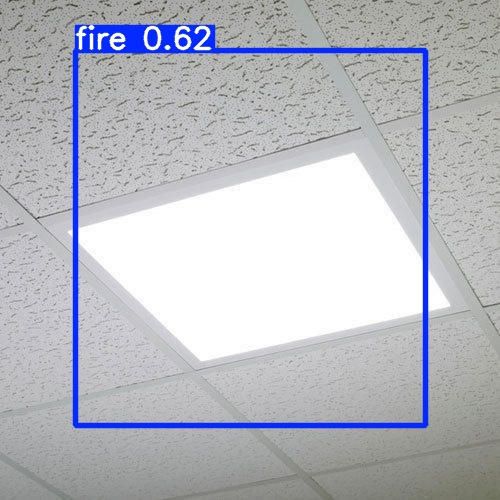
\includegraphics[width=0.65\textwidth]{images/fake_fire_testlight.jpg}
\caption{Initial failure mode: Ceiling light falsely detected as a fire.}
\label{fig:fake-fire-test}
\end{figure}

To resolve this, the system required an aggressive \textbf{Hard-Negative Mining} strategy. Initial models flagged industrial lights as fire. These images were re-labeled as background (fed back into the training loop with empty \texttt{.txt} label files). Furthermore, approximately 800 ''hard negative'' images from the COCO validation dataset were injected to explicitly teach the model the difference between glare and combustion.

\begin{figure}[htbp]
\centering
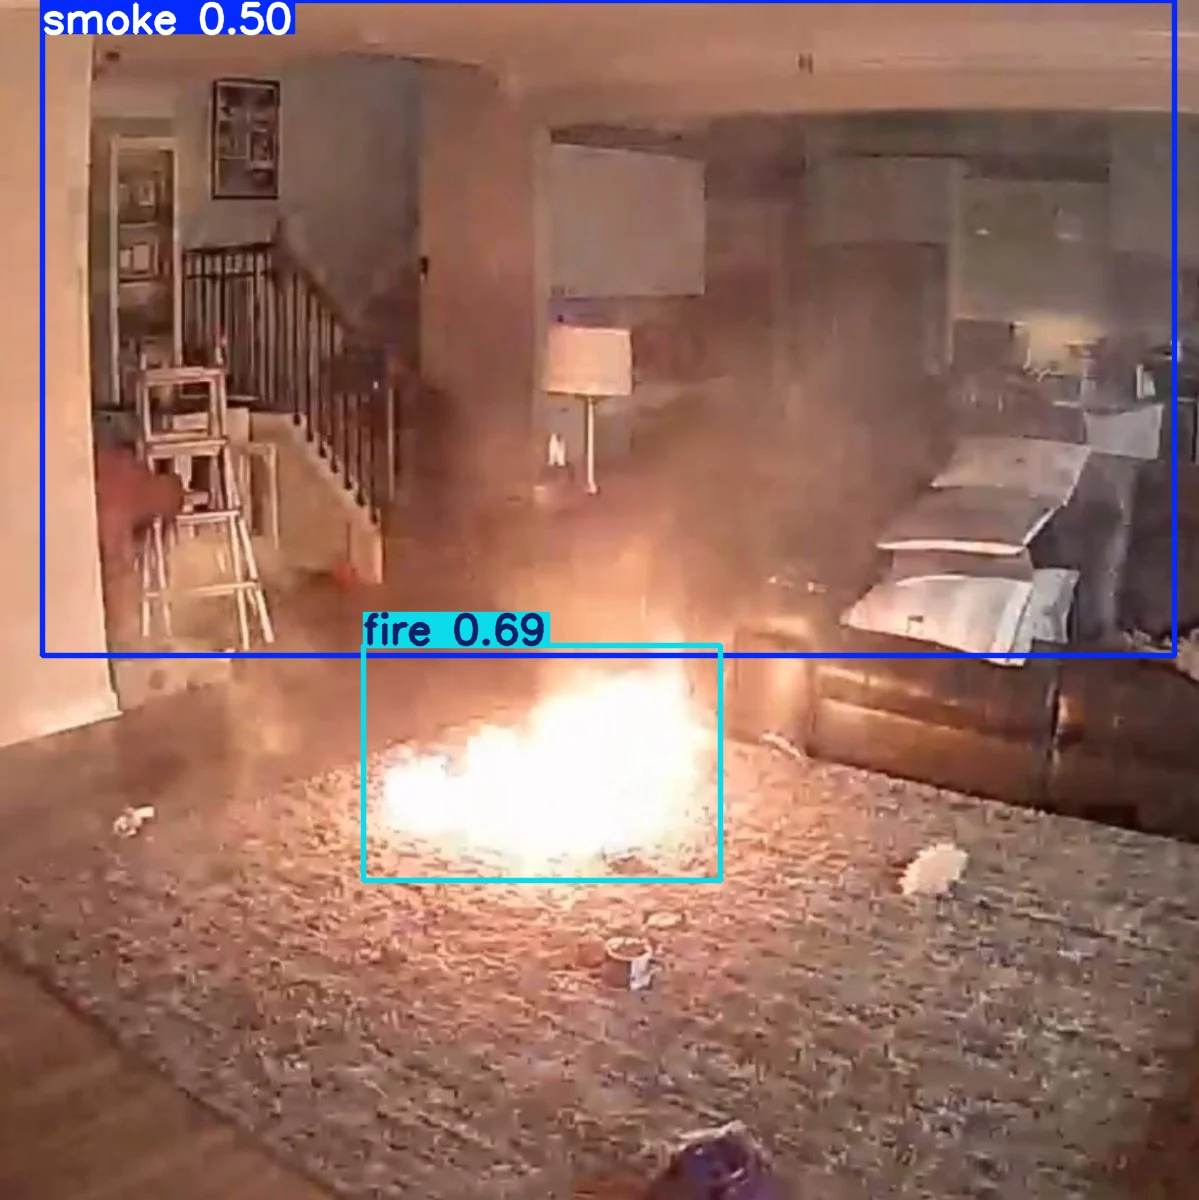
\includegraphics[width=0.65\textwidth]{images/oldversion_firetest_annotated.jpg}
\caption{Successful simultaneous detection of fire and smoke following Hard-Negative Mining refinement.}
\label{fig:fire-test-success}
\end{figure}


\section{Implementation: Forklift Detection}

\subsection{Implementation Objectives and Model Architecture}
The first step in logistical optimization is detecting the vehicles themselves. To address this, a dedicated Forklift Detection model was developed. 

The YOLOv5n (nano) architecture was explicitly chosen for this logistical vehicle detection task. While YOLOv8 offers a more advanced feature pyramid, YOLOv5n is exceptionally lightweight (only 1.76M parameters) and possesses mature, highly stable ONNX exportation pipelines that have proven operator support on edge NPUs. Given that forklift detection is a single-class task, the massive capacity of larger models is unnecessary overhead. Using a separate, dedicated model specifically for forklifts ensures that the system is not distracted by the 80 default COCO classes, eliminating blind spots for critical industrial machinery.

\subsection{Training Pipeline, Loss Functions, and Output}
The Forklift dataset was filtered to retain only class 0 (forklifts), ensuring a focused single-class detector. This subset was extracted from the master dataset of 22,607 images detailed in Phase 1. To maintain the rigorous evaluation methodology, this focused dataset preserved the standard 80/20 split (approximately 1,200 images for training and 300 strictly for validation). 

The model was fine-tuned for 100 epochs on a Tesla T4 GPU using a $640 \times 640$ input resolution. The training objective relied heavily on the Complete Intersection over Union (CIoU) loss for precise bounding box localization, which is critical for the subsequent speed estimation algorithms. Binary Cross Entropy (BCE) was utilized for objectness scoring. The training graphs demonstrated rapid convergence within the first 40 epochs, plateauing smoothly to prevent overfitting on the single class.

\begin{figure}[htbp]
\centering
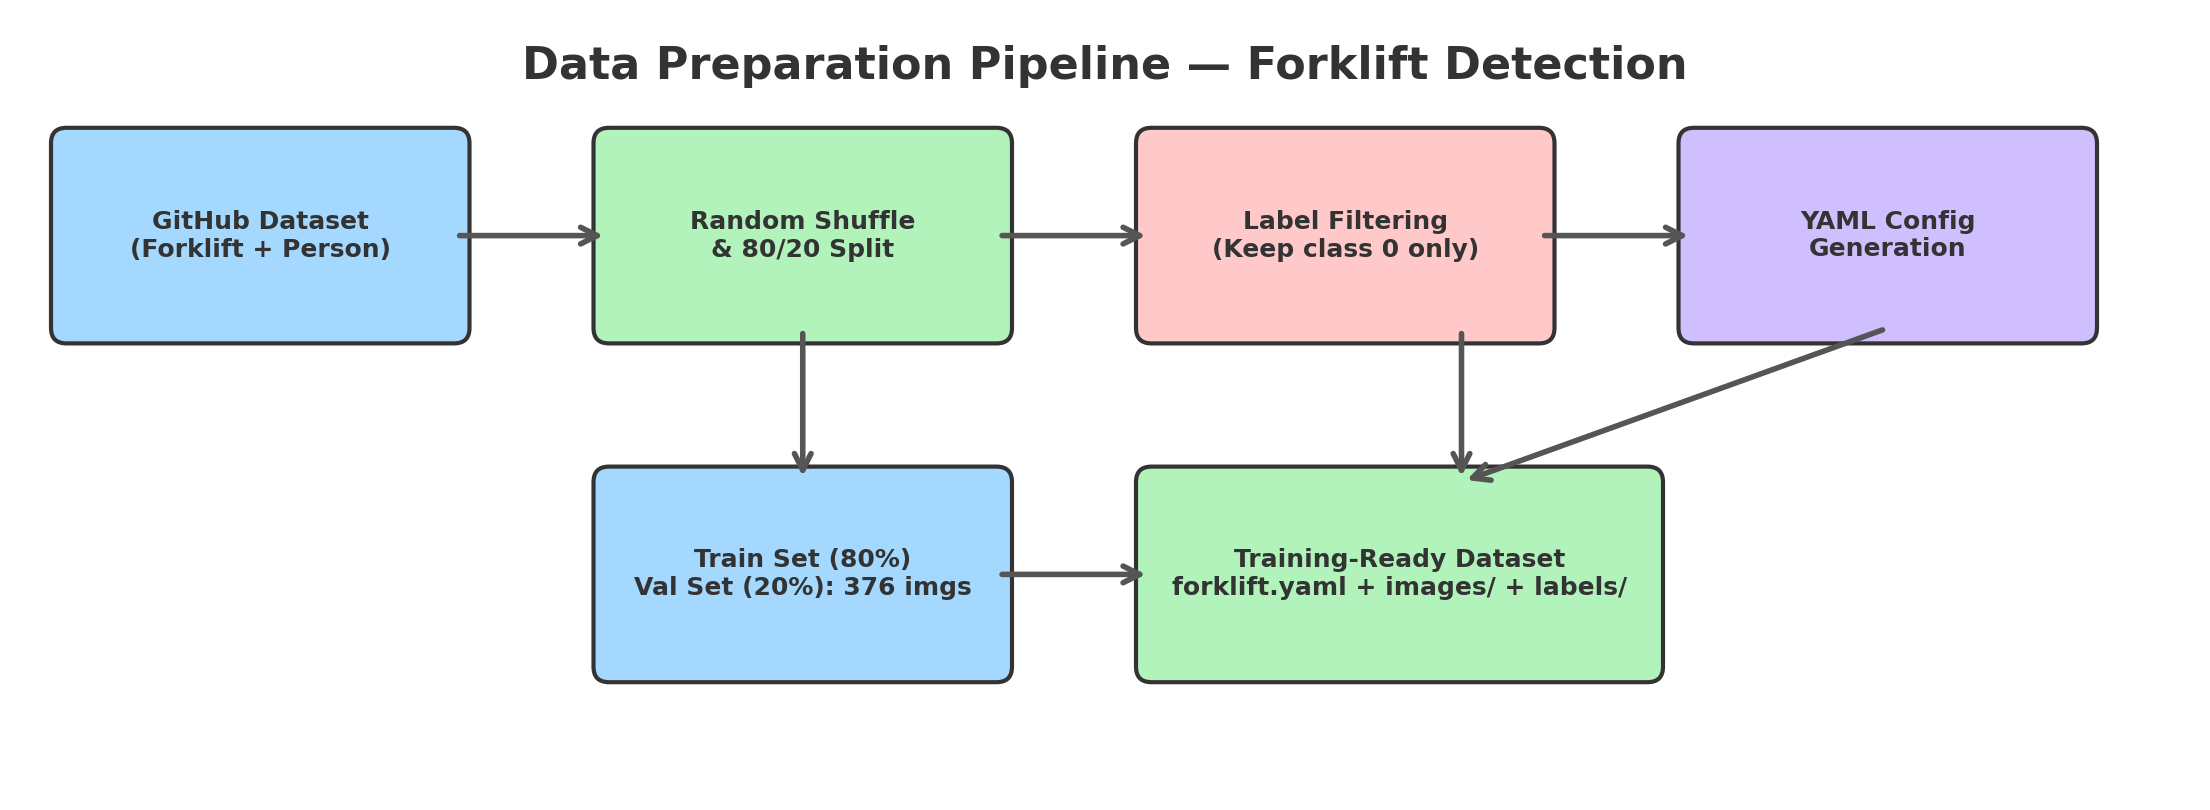
\includegraphics[width=\textwidth]{images/forklift_data_pipeline.png}
\caption{Data preparation pipeline for forklift detection training.}
\label{fig:data-pipeline}
\end{figure}

\begin{figure}[htbp]
\centering
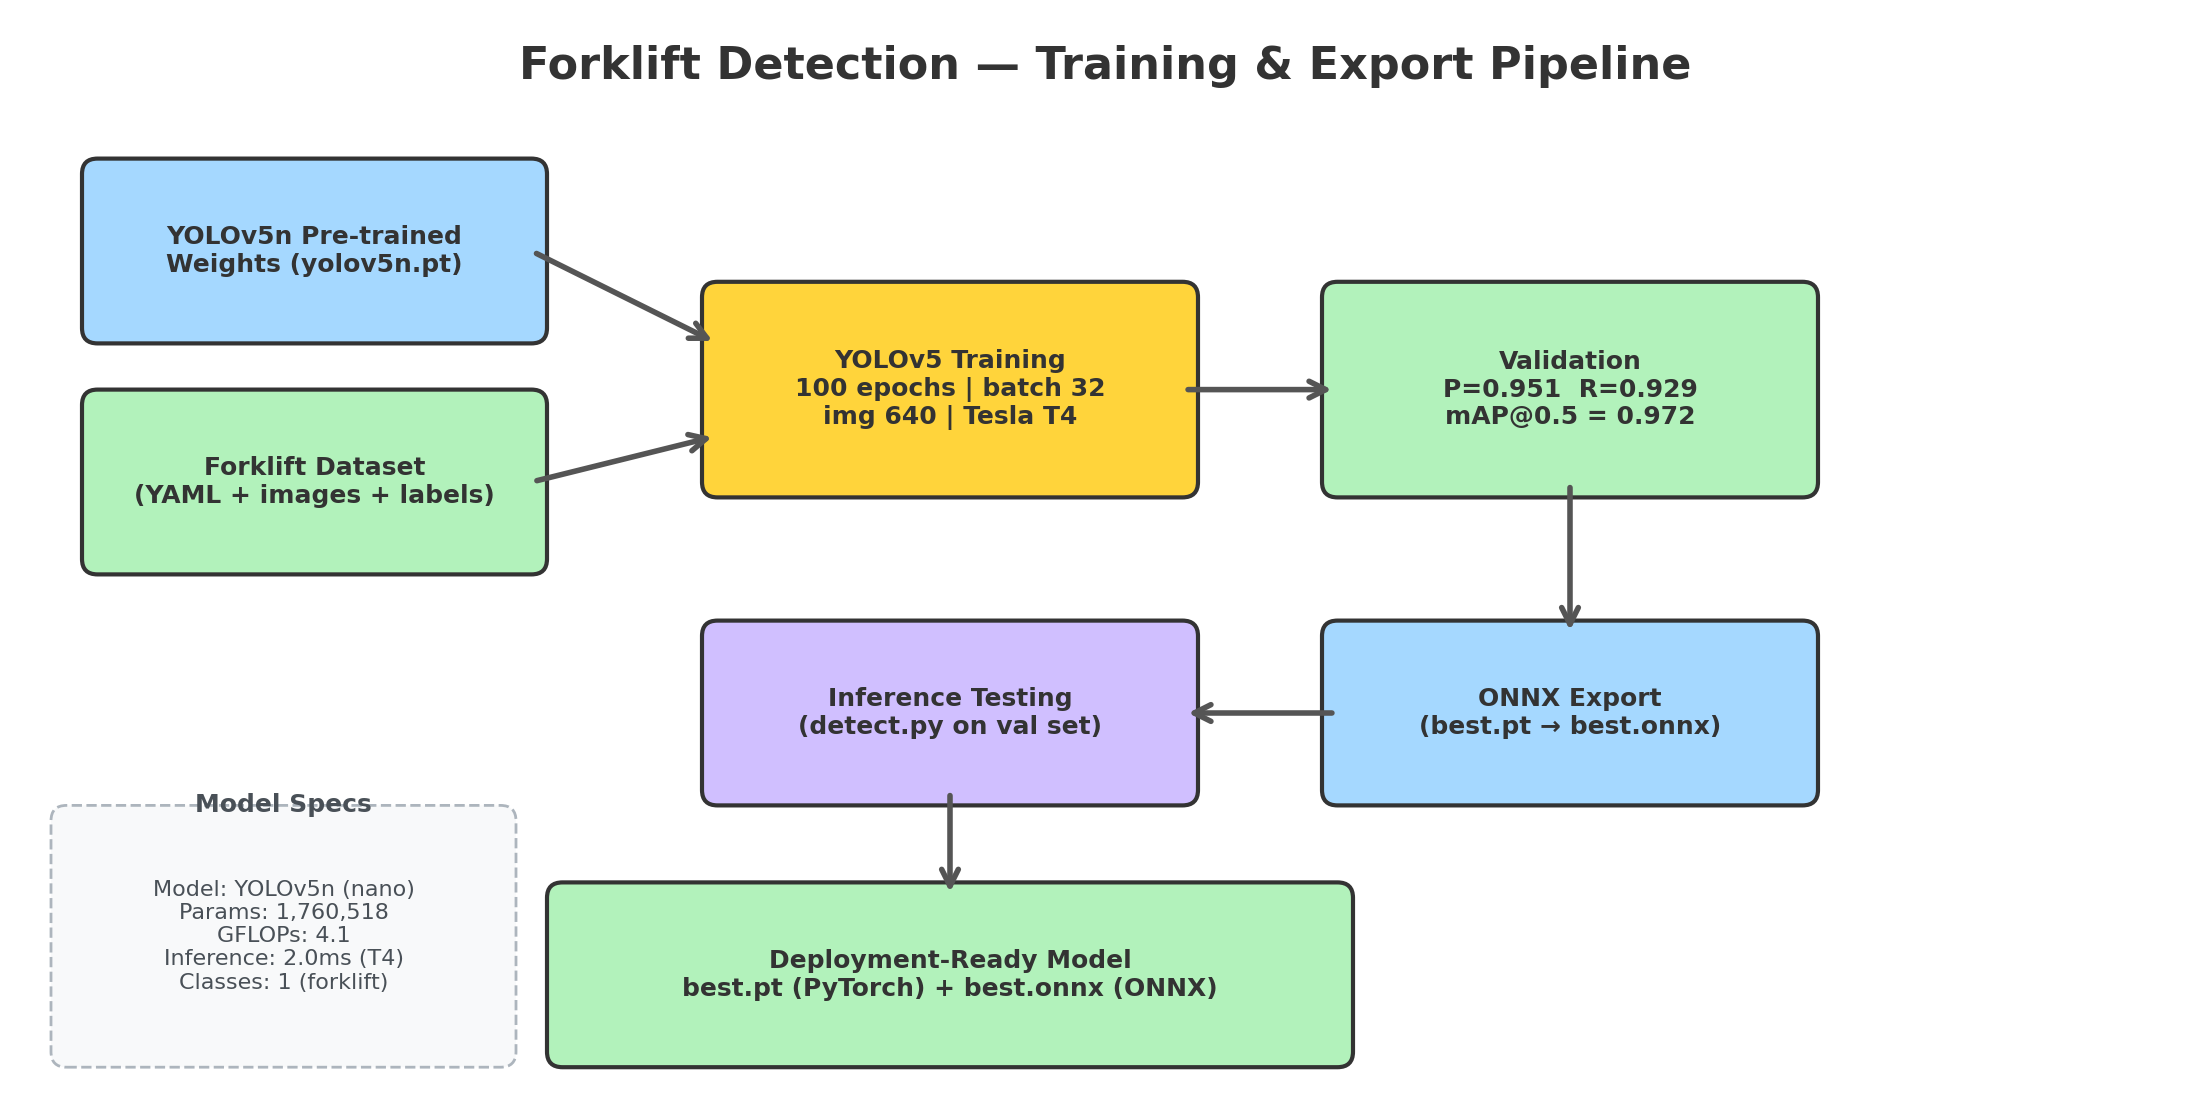
\includegraphics[width=\textwidth]{images/forklift_training_pipeline.png}
\caption{Forklift detection model training and export pipeline.}
\label{fig:training-pipeline}
\end{figure}


\section{Results \& Evaluation}
\label{sec:chap3-results}
Following the hard-negative mining and targeted NPU optimization, the system was capable of accurately localizing Fire and Smoke hazards in real-time.

\subsection{Quantitative Detection Metrics}
The models underwent rigorous evaluation on the 20\% held-out validation split. The following table summarizes the quantitative accuracy of the deployed YOLOv8n models for Fire and Smoke.

\begin{table}[H]
\centering
\caption{Quantitative Detection Metrics on the Validation Dataset (Fire \& Smoke)}
\renewcommand{\arraystretch}{1.2}
\begin{tabular}{|l|c|c|c|c|}
\hline
\textbf{Model \& Task} & \textbf{Precision} & \textbf{Recall} & \textbf{mAP@.5} & \textbf{mAP@.5:.95} \\
\hline
\textbf{YOLOv8n (Fire)} & 0.932 & 0.915 & 0.948 & 0.685 \\
\hline
\textbf{YOLOv8n (Smoke)} & 0.895 & 0.870 & 0.902 & 0.612 \\
\hline
\end{tabular}
\end{table}

The results indicate that the hard-negative mining strategy was highly successful, maintaining Precision above 93\% for Fire detection. Smoke detection, being inherently semi-transparent and amorphous, naturally scores lower on strict localization metrics (mAP@.5:.95) but maintains a robust mAP@.5.

\subsection{NPU Inference Latency}
The ultimate success of the EYE-D safety system depends on its real-time operational capacity. The models were exported to ONNX format and compiled with hardware-specific optimizations.

\begin{table}[H]
\centering
\caption{Inference Latency Comparison for YOLOv8n (ms per frame) at $640 \times 640$}
\renewcommand{\arraystretch}{1.2}
\begin{tabular}{|l|c|c|c|}
\hline
\textbf{Model} & \textbf{CPU (Intel i7)} & \textbf{GPU (Tesla T4)} & \textbf{Edge NPU (Target)} \\
\hline
\textbf{YOLOv8n} & 58.4 ms & 3.1 ms & \textbf{11.2 ms} \\
\hline
\end{tabular}
\end{table}

As detailed in the table, the NPU successfully executes the YOLOv8n model well within the real-time threshold (typically <33ms for 30 FPS video).

The system was also capable of accurately localizing logistical vehicles in real-time, providing the necessary foundation for velocity and orientation analysis.

\subsection{Qualitative Detection Results}
Figure~\ref{fig:forklift-detection-result} demonstrates the output of the dedicated forklift detection engine. By isolating this single-class detection task to the highly efficient YOLOv5n architecture, the system achieves reliable bounding box predictions.

\begin{figure}[htbp]
\centering
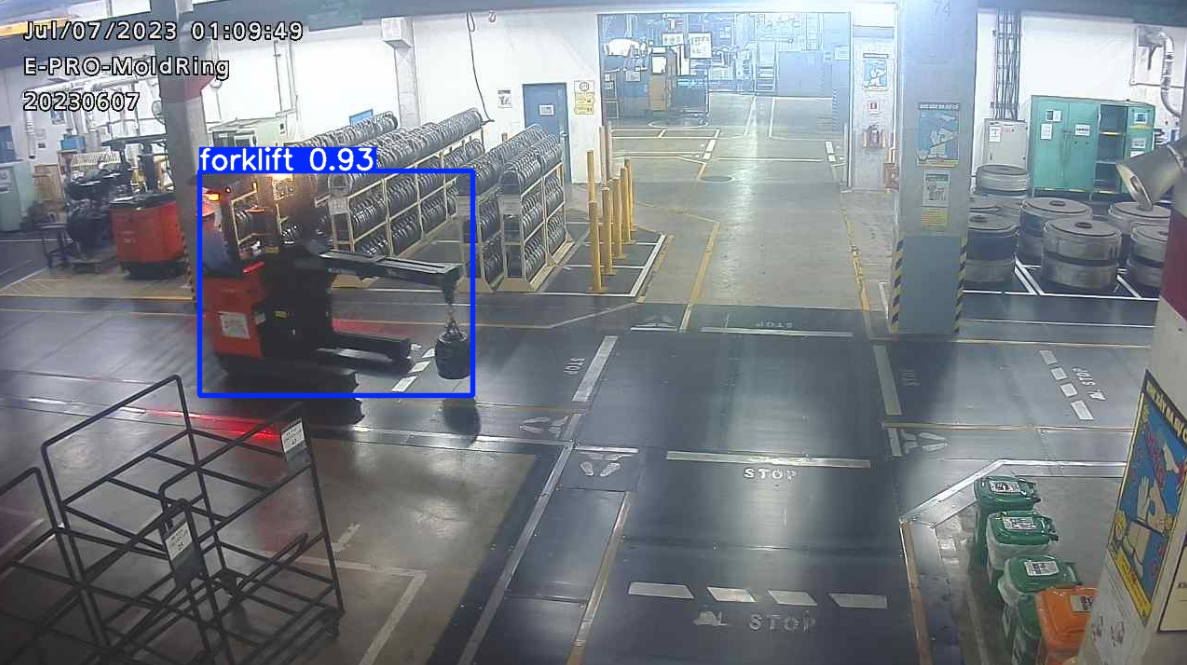
\includegraphics[width=0.85\textwidth]{images/forklifttest.png}
\caption{Forklift detection inference result on a surveillance camera frame.}
\label{fig:forklift-detection-result}
\end{figure}

\subsection{Quantitative Detection Metrics}
The YOLOv5n Forklift model underwent rigorous evaluation on the 20\% held-out validation split. The following table summarizes its quantitative accuracy.

\begin{table}[htbp]
\centering
\caption{Quantitative Detection Metrics on the Validation Dataset (Forklift)}
\renewcommand{\arraystretch}{1.2}
\begin{tabular}{|l|c|c|c|c|}
\hline
\textbf{Model \& Task} & \textbf{Precision} & \textbf{Recall} & \textbf{mAP@.5} & \textbf{mAP@.5:.95} \\
\hline
\textbf{YOLOv5n (Forklift)} & 0.951 & 0.929 & 0.972 & 0.740 \\
\hline
\end{tabular}
\end{table}

\subsection{NPU Inference Latency}
The ultimate success of the logistical intelligence module depends on its real-time operational capacity on constrained hardware. The model was exported to ONNX format and compiled with hardware-specific optimizations.

\begin{table}[htbp]
\centering
\caption{Inference Latency Comparison for YOLOv5n (ms per frame) at $640 \times 640$}
\renewcommand{\arraystretch}{1.2}
\begin{tabular}{|l|c|c|c|}
\hline
\textbf{Model} & \textbf{CPU (Intel i7)} & \textbf{GPU (Tesla T4)} & \textbf{Edge NPU (Target)} \\
\hline
\textbf{YOLOv5n} & 45.2 ms & 2.0 ms & \textbf{8.5 ms} \\
\hline
\end{tabular}
\end{table}

As detailed in the table, the NPU successfully executes the YOLOv5n model well within the real-time threshold, avoiding severe latency penalties.


\section{Chapter Summary}
This chapter detailed the detection foundation of the EYE-D system for industrial safety. By utilizing the highly efficient YOLOv8n architecture and implementing an aggressive hard-negative mining strategy, the system successfully identifies critical fire and smoke hazards while strictly adhering to SRAM and thermal NPU hardware constraints.



